\documentclass[aspectratio=169]{beamer}

% ── Theme & Colours ──────────────────────────────────────────────────────────
\usetheme{Madrid}
\usecolortheme{default}

\definecolor{navyblue}{RGB}{26,31,54}
\definecolor{electricblue}{RGB}{79,110,247}
\definecolor{lightblue}{RGB}{220,230,255}
\definecolor{successgreen}{RGB}{34,197,94}
\definecolor{warnorange}{RGB}{245,158,11}
\definecolor{softgray}{RGB}{248,249,252}

\setbeamercolor{palette primary}{bg=navyblue, fg=white}
\setbeamercolor{palette secondary}{bg=electricblue, fg=white}
\setbeamercolor{palette tertiary}{bg=navyblue!80, fg=white}
\setbeamercolor{palette quaternary}{bg=navyblue, fg=white}
\setbeamercolor{structure}{fg=navyblue}
\setbeamercolor{section in toc}{fg=navyblue}
\setbeamercolor{frametitle}{bg=navyblue, fg=white}
\setbeamercolor{title}{fg=white}
\setbeamercolor{subtitle}{fg=lightblue}
\setbeamercolor{author}{fg=lightblue}
\setbeamercolor{date}{fg=lightblue}
\setbeamercolor{institute}{fg=lightblue}
\setbeamercolor{block title}{bg=electricblue, fg=white}
\setbeamercolor{block body}{bg=lightblue!40, fg=navyblue}
\setbeamercolor{block title alerted}{bg=red!70!black, fg=white}
\setbeamercolor{block body alerted}{bg=red!10, fg=black}
\setbeamercolor{block title example}{bg=successgreen!80!black, fg=white}
\setbeamercolor{block body example}{bg=successgreen!10, fg=black}
\setbeamercolor{itemize item}{fg=electricblue}
\setbeamercolor{itemize subitem}{fg=navyblue!70}
\setbeamercolor{enumerate item}{fg=electricblue}

\setbeamertemplate{itemize item}{\scriptsize\raise1.5pt\hbox{\donotcoloroutermaths$\blacktriangleright$}}
\setbeamertemplate{itemize subitem}{\tiny\raise1.5pt\hbox{\donotcoloroutermaths$\bullet$}}
\setbeamertemplate{navigation symbols}{}
\setbeamertemplate{footline}{
  \leavevmode%
  \hbox{%
    \begin{beamercolorbox}[wd=.30\paperwidth,ht=2.5ex,dp=1.5ex,left,leftskip=1mm]{palette primary}%
      \usebeamerfont{author in head/foot}\insertshortauthor
    \end{beamercolorbox}%
    \begin{beamercolorbox}[wd=.40\paperwidth,ht=2.5ex,dp=1.5ex,center]{palette secondary}%
      \usebeamerfont{title in head/foot}\insertshorttitle
    \end{beamercolorbox}%
    \begin{beamercolorbox}[wd=.30\paperwidth,ht=2.5ex,dp=1.5ex,right,rightskip=1mm]{palette primary}%
      \usebeamerfont{date in head/foot}\insertframenumber{} / \inserttotalframenumber
    \end{beamercolorbox}%
  }
}

% ── Packages ─────────────────────────────────────────────────────────────────
\usepackage{amsmath,amssymb}
\usepackage{graphicx}
\usepackage{booktabs}
\usepackage{array}
\usepackage{colortbl}
\usepackage{xcolor}
\usepackage{tikz}
\usetikzlibrary{shapes.geometric, arrows.meta, positioning, fit, backgrounds, shadows.blur}
\usepackage{tcolorbox}
\tcbuselibrary{skins,breakable}
\usepackage{svg}
\svgsetup{inkscapelatex=false}
\usepackage{pgfplots}
\pgfplotsset{compat=1.18}
\usepackage{multicol}

\hbadness=10000
\vbadness=10000
\hfuzz=10pt
\vfuzz=200pt

% ── Shared tcolorbox styles ───────────────────────────────────────────────────
\tcbset{
  bluebox/.style={colback=electricblue!12, colframe=electricblue,
    fonttitle=\small\bfseries, boxrule=1.2pt, left=4pt, right=4pt,
    top=3pt, bottom=3pt},
  greenbox/.style={colback=successgreen!10, colframe=successgreen!70!black,
    fonttitle=\small\bfseries, boxrule=1.2pt, left=4pt, right=4pt,
    top=3pt, bottom=3pt},
  orangebox/.style={colback=warnorange!12, colframe=warnorange,
    fonttitle=\small\bfseries, boxrule=1.2pt, left=4pt, right=4pt,
    top=3pt, bottom=3pt},
  redbox/.style={colback=red!8, colframe=red!65!black,
    fonttitle=\small\bfseries, boxrule=1.2pt, left=4pt, right=4pt,
    top=3pt, bottom=3pt},
  navybox/.style={colback=navyblue!8, colframe=navyblue,
    fonttitle=\small\bfseries, boxrule=1.2pt, left=4pt, right=4pt,
    top=3pt, bottom=3pt},
}

% ── TikZ Styles ──────────────────────────────────────────────────────────────
\tikzset{
  component/.style={rectangle, rounded corners=4pt, draw=navyblue, thick,
    fill=lightblue!60, text=navyblue, font=\small\bfseries,
    minimum height=0.7cm, minimum width=2.2cm, align=center},
  arrow/.style={-Stealth, thick, color=electricblue},
  flow/.style={rectangle, rounded corners=3pt, draw=navyblue!70, thick,
    fill=white, text=navyblue, font=\footnotesize, align=center,
    minimum height=0.6cm, minimum width=1.8cm},
}

% ── Metadata ─────────────────────────────────────────────────────────────────
\title[SecureFileShare]{Secure Decentralised File Sharing}
\subtitle{Using Blockchain \& IPFS}
\author[IT352 Project]{Aadharsh~Ramachandran and Paluvadi~Dinesh~Manideep}
\institute[Thakur / Universal College]{IT352 Information Assurance and Security End Evaluation}


% =============================================================================
\begin{document}
% =============================================================================

% ── Title Slide ───────────────────────────────────────────────────────────────
\begin{frame}[plain]
\begin{tikzpicture}[remember picture, overlay]
  \fill[navyblue] (current page.north west) rectangle (current page.south east);
  \fill[electricblue, opacity=0.18]
    (current page.north east)
    .. controls +(-3,-2) and +(2,2) ..
    ([xshift=-3cm]current page.east)
    -- (current page.south east) -- cycle;
\end{tikzpicture}
\vspace{0.4cm}
\titlepage
\end{frame}

% ── Outline ───────────────────────────────────────────────────────────────────
\begin{frame}{Presentation Outline}
\begin{tcolorbox}[navybox, title=\textbf{Outline}]
\small
\begin{enumerate}
  \item Introduction \& Problem Statement
  \item Objectives
  \item Novel Contributions
  \item Methodology \& Algorithm
  \item System Architecture
  \item Results \& Analysis
  \item Post-Mid ZK Enhancements
\end{enumerate}
\end{tcolorbox}
\end{frame}

% =============================================================================
\section{Introduction \& Problem Statement}
% =============================================================================

\begin{frame}{Introduction --- The Digital Storage Crisis}
\begin{tcolorbox}[redbox, title=\textbf{Core Problem}]
\small
Traditional file sharing systems rely on central servers that are single points of failure ---
vulnerable to data breaches, unauthorized access, and provider misuse. They offer no
cryptographic guarantees over who can access files, for how long, or whether data is truly
deleted when requested --- fundamental, unresolved security risks that grow with every
terabyte stored.
\end{tcolorbox}
\vspace{0.18cm}
\begin{tcolorbox}[bluebox, title=\textbf{Limitations of Centralised Storage}]
\scriptsize
\begin{columns}[t]
\column{0.48\textwidth}
\begin{itemize}
  \item \textbf{Single Point of Failure} --- one breach exposes everything
  \item \textbf{Third-Party Dependency} --- loss of data ownership
  \item \textbf{No Tamper Evidence} --- silent data manipulation possible
\end{itemize}
\column{0.48\textwidth}
\begin{itemize}
  \item \textbf{High Operational Costs} --- centralised infrastructure scales poorly
  \item \textbf{Availability Issues} --- server downtime = inaccessible data
  \item \textbf{Privacy Violations} --- provider retains unilateral access
\end{itemize}
\end{columns}
\end{tcolorbox}
\end{frame}

\begin{frame}{Problem Statement}
\begin{tcolorbox}[redbox, title={\textbf{Problem Statement}}]
\small
How can organisations securely share confidential files over an untrusted network
\textbf{without relying on any central authority}, while simultaneously guaranteeing
\textbf{data integrity}, \textbf{fine-grained cryptographic access control},
\textbf{legal compliance (GDPR)}, and \textbf{mathematical verifiability of access}?
\end{tcolorbox}
\vspace{0.2cm}
\begin{columns}[t]
\column{0.48\textwidth}
\begin{tcolorbox}[bluebox, title=\textbf{What Existing Solutions Miss}]
\small
\begin{itemize}
  \item No privacy-preserving anonymous access verification flow
  \item Rigid access control (all-or-nothing permissions)
\end{itemize}
\end{tcolorbox}
\column{0.48\textwidth}
\begin{tcolorbox}[greenbox, title=\textbf{What Existing Solutions Miss}]
\small
\begin{itemize}
  \item GDPR ``Right to Erasure'' vs. blockchain immutability paradox
  \item Permissions do not expire automatically
  \item Weak integration between on-chain policy and off-chain storage
\end{itemize}
\end{tcolorbox}
\end{columns}
\end{frame}

% =============================================================================
\section{Objectives}
% =============================================================================

\begin{frame}{Research Objectives}
\begin{columns}[t]
\column{0.48\textwidth}
\begin{tcolorbox}[redbox, title=\textbf{Security Objectives}]
\scriptsize
\begin{itemize}
  \item[\textbf{O1}] Encrypt files with \textbf{AES-256-GCM} before any storage
  \item[\textbf{O2}] Verify chunk integrity via \textbf{SHA-256} hashing
  \item[\textbf{O3}] Enforce anonymous access checks using \textbf{Semaphore proofs}
  \item[\textbf{O4}] Support \textbf{CP-ABE} policy encryption with safe fallback mode
  \item[\textbf{O5}] Achieve \textbf{GDPR compliance} (Articles 17 \& 20) in Web3
\end{itemize}
\end{tcolorbox}
\column{0.48\textwidth}
\begin{tcolorbox}[bluebox, title=\textbf{Storage Objectives}]
\scriptsize
\begin{itemize}
  \item[\textbf{O6}] Store encrypted chunks on \textbf{IPFS} with CID-based addressing
  \item[\textbf{O7}] Register file metadata immutably on \textbf{Ethereum blockchain}
  \item[\textbf{O8}] Keep backend-state consistency with on-chain file and policy state
\end{itemize}
\end{tcolorbox}
\vspace{0.15cm}
\begin{tcolorbox}[greenbox, title=\textbf{Governance Objectives}]
\scriptsize
\begin{itemize}
  \item[\textbf{O9}] Automate ABAC and ZK policy checks via smart contracts
  \item[\textbf{O10}] Enforce \textbf{time-bound permissions} using \texttt{block.timestamp}
\end{itemize}
\end{tcolorbox}
\end{columns}
\end{frame}

% =============================================================================
\section{Novel Contributions}
% =============================================================================

\begin{frame}{Four Novel Contributions}
\begin{columns}[T]
\column{0.48\textwidth}
\begin{tcolorbox}[bluebox, title=\textbf{N1: Zero-Knowledge Proofs (ZKP)},
  height=5.8cm, valign=top]
\scriptsize
\textbf{Implementation path:} Semaphore + \texttt{FileAccessControl.sol}\\[5pt]
\textbf{Core behavior:}
\begin{itemize}
  \item Anonymous proof validation through Semaphore groups
  \item File access proof uses file-bound message semantics
  \item Leader-proof path controls ZK group member onboarding
\end{itemize}
\textbf{Impact:} Privacy-preserving access verification without exposing identity attributes
\end{tcolorbox}
\column{0.48\textwidth}
\begin{tcolorbox}[greenbox, title=\textbf{N2: Attribute-Based Encryption (ABE)},
  height=5.8cm, valign=top]
\scriptsize
\textbf{Implemented path:}
\begin{itemize}
  \item CP-ABE service for attribute-driven key protection
  \item ECDH + HKDF key wrapping for direct share flow
  \item Safe runtime fallback if CP-ABE binaries are unavailable
\end{itemize}
\textbf{Impact:} Fine-grained cryptographic key access based on attributes/policies
\end{tcolorbox}
\end{columns}
\end{frame}

\begin{frame}{Four Novel Contributions}
\begin{columns}[T]
\column{0.48\textwidth}
\begin{tcolorbox}[orangebox, title=\textbf{N3: Time-Bound Permissions},
  height=5.8cm, valign=top]
\scriptsize
\textbf{Contract:} \texttt{TimeBoundPermissions.sol}\\[5pt]
\textbf{Implemented support:}
\begin{itemize}
  \item Grant temporary access with explicit expiry
  \item Extend/revoke permission lifecycle
  \item Runtime checks enforce valid access window
\end{itemize}
\textbf{Impact:} Automatic expiry reduces stale/over-privileged access risk
\end{tcolorbox}
\column{0.48\textwidth}
\begin{tcolorbox}[redbox, title=\textbf{N4: GDPR Compliance Module},
  height=5.8cm, valign=top]
\scriptsize
\textbf{Hybrid approach:}
\begin{itemize}
  \item Erasure/export APIs with SQLite operational records
  \item On-chain compliance signaling via \texttt{GDPRCompliance.sol}
  \item Storage cleanup and audit trace across off-chain/on-chain layers
\end{itemize}
\textbf{Impact:} Practical legal-compliance trail in decentralized file lifecycle
\end{tcolorbox}
\end{columns}
\end{frame}

% =============================================================================
\section{Methodology}
% =============================================================================

\begin{frame}{Methodology --- End-to-End Algorithm}
\begin{columns}[c]
\column{0.52\textwidth}
\begin{tcolorbox}[navybox, title=\textbf{Algorithm Steps (Implemented)}]
\scriptsize
\begin{enumerate}
  \item[\textbf{S1}] \textbf{Auth + Identity Setup} --- wallet signature auth and local Semaphore identity
  \item[\textbf{S2}] \textbf{Encrypt File} --- AES-256-GCM (64KB chunks) + SHA-256 hashes
  \item[\textbf{S3}] \textbf{Store on IPFS} --- upload encrypted chunks and receive CIDs
  \item[\textbf{S4}] \textbf{On-chain Register} --- \texttt{FileRegistry} + ownership/policy registration
  \item[\textbf{S5}] \textbf{Branch A (Without ZK)} --- normal group / ABAC / timed-permission checks
  \item[\textbf{S6}] \textbf{Branch B (With ZK)} --- Semaphore proof validation + ZK group policy checks
  \item[\textbf{S7}] \textbf{Compliance} --- erasure/export workflow with audit records
\end{enumerate}
\end{tcolorbox}

\column{0.43\textwidth}
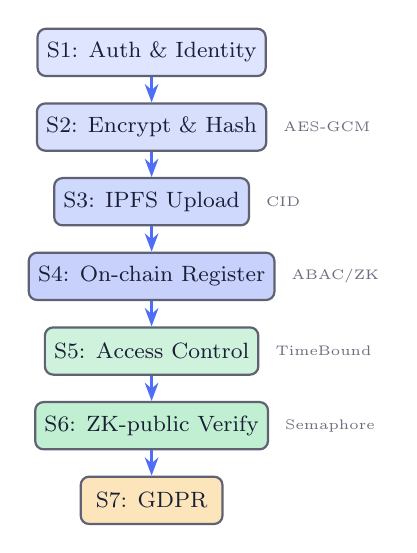
\begin{tikzpicture}[node distance=0.32cm]
  \node[flow, fill=electricblue!18] (s1) {S1: Auth \& Identity};
  \node[flow, fill=electricblue!22, below=of s1] (s2) {S2: Encrypt \& Hash};
  \node[flow, fill=electricblue!27, below=of s2] (s3) {S3: IPFS Upload};
  \node[flow, fill=electricblue!32, below=of s3] (s4) {S4: On-chain Register};
  \node[flow, fill=successgreen!22, below=of s4] (s5) {S5: Access Control};
  \node[flow, fill=successgreen!28, below=of s5] (s6) {S6: ZK-public Verify};
  \node[flow, fill=warnorange!28, below=of s6] (s7) {S7: GDPR};
  \draw[arrow] (s1)--(s2); \draw[arrow] (s2)--(s3);
  \draw[arrow] (s3)--(s4); \draw[arrow] (s4)--(s5);
  \draw[arrow] (s5)--(s6); \draw[arrow] (s6)--(s7);
  \node[right=0.08cm of s2, font=\tiny, text=navyblue!65] {AES-GCM};
  \node[right=0.08cm of s3, font=\tiny, text=navyblue!65] {CID};
  \node[right=0.08cm of s4, font=\tiny, text=navyblue!65] {ABAC/ZK};
  \node[right=0.08cm of s5, font=\tiny, text=navyblue!65] {TimeBound};
  \node[right=0.08cm of s6, font=\tiny, text=navyblue!65] {Semaphore};
\end{tikzpicture}
\end{columns}
\end{frame}

\begin{frame}{Cryptographic Pipeline in Detail}
\begin{columns}[t]
\column{0.48\textwidth}
\begin{tcolorbox}[bluebox, title=\textbf{File Encryption (AES-256-GCM)}]
\tiny
\begin{enumerate}
  \item Generate random 256-bit AES key
  \item Split file into \textbf{64\,KB chunks}
  \item Per chunk: 96-bit IV $\to$ GCM cipher $\to$ auth-tag
  \item SHA-256(plaintext chunk) stored for integrity checking
  \item Upload encrypted chunks to IPFS $\to$ array of CIDs
  \item Register CIDs + file hash on \texttt{FileRegistry.sol}
\end{enumerate}
\end{tcolorbox}
\vspace{0.12cm}
\begin{tcolorbox}[navybox, title=\textbf{Key Share / Wrap Paths}]
\tiny
\begin{itemize}
  \item ECDH + HKDF key wrapping for direct share flows
  \item CP-ABE service available with runtime fallback if binaries are absent
\end{itemize}
\end{tcolorbox}
\column{0.48\textwidth}
\begin{tcolorbox}[bluebox, title=\textbf{Semaphore-based ZK Access Flow}]
\scriptsize
\begin{enumerate}
  \item Build proof with file-bound message (or leader-member-add message)
  \item Validate proof on Semaphore via relayer/direct tx path
  \item Backend verifies receipt/log semantics for ZK-public download
\end{enumerate}
\end{tcolorbox}
\vspace{0.12cm}
\begin{tcolorbox}[greenbox, title=\textbf{GDPR Erasure Pipeline}]
\scriptsize
\texttt{/api/gdpr/erase} $\to$ storage cleanup + DB updates $\to$
\texttt{GDPRCompliance.sol} signaling and auditable records
\end{tcolorbox}
\end{columns}
\end{frame}

% =============================================================================
\section{System Architecture}
% =============================================================================

\begin{frame}[plain]
\centering
\IfFileExists{securefile_architecture_flow.png}{%
  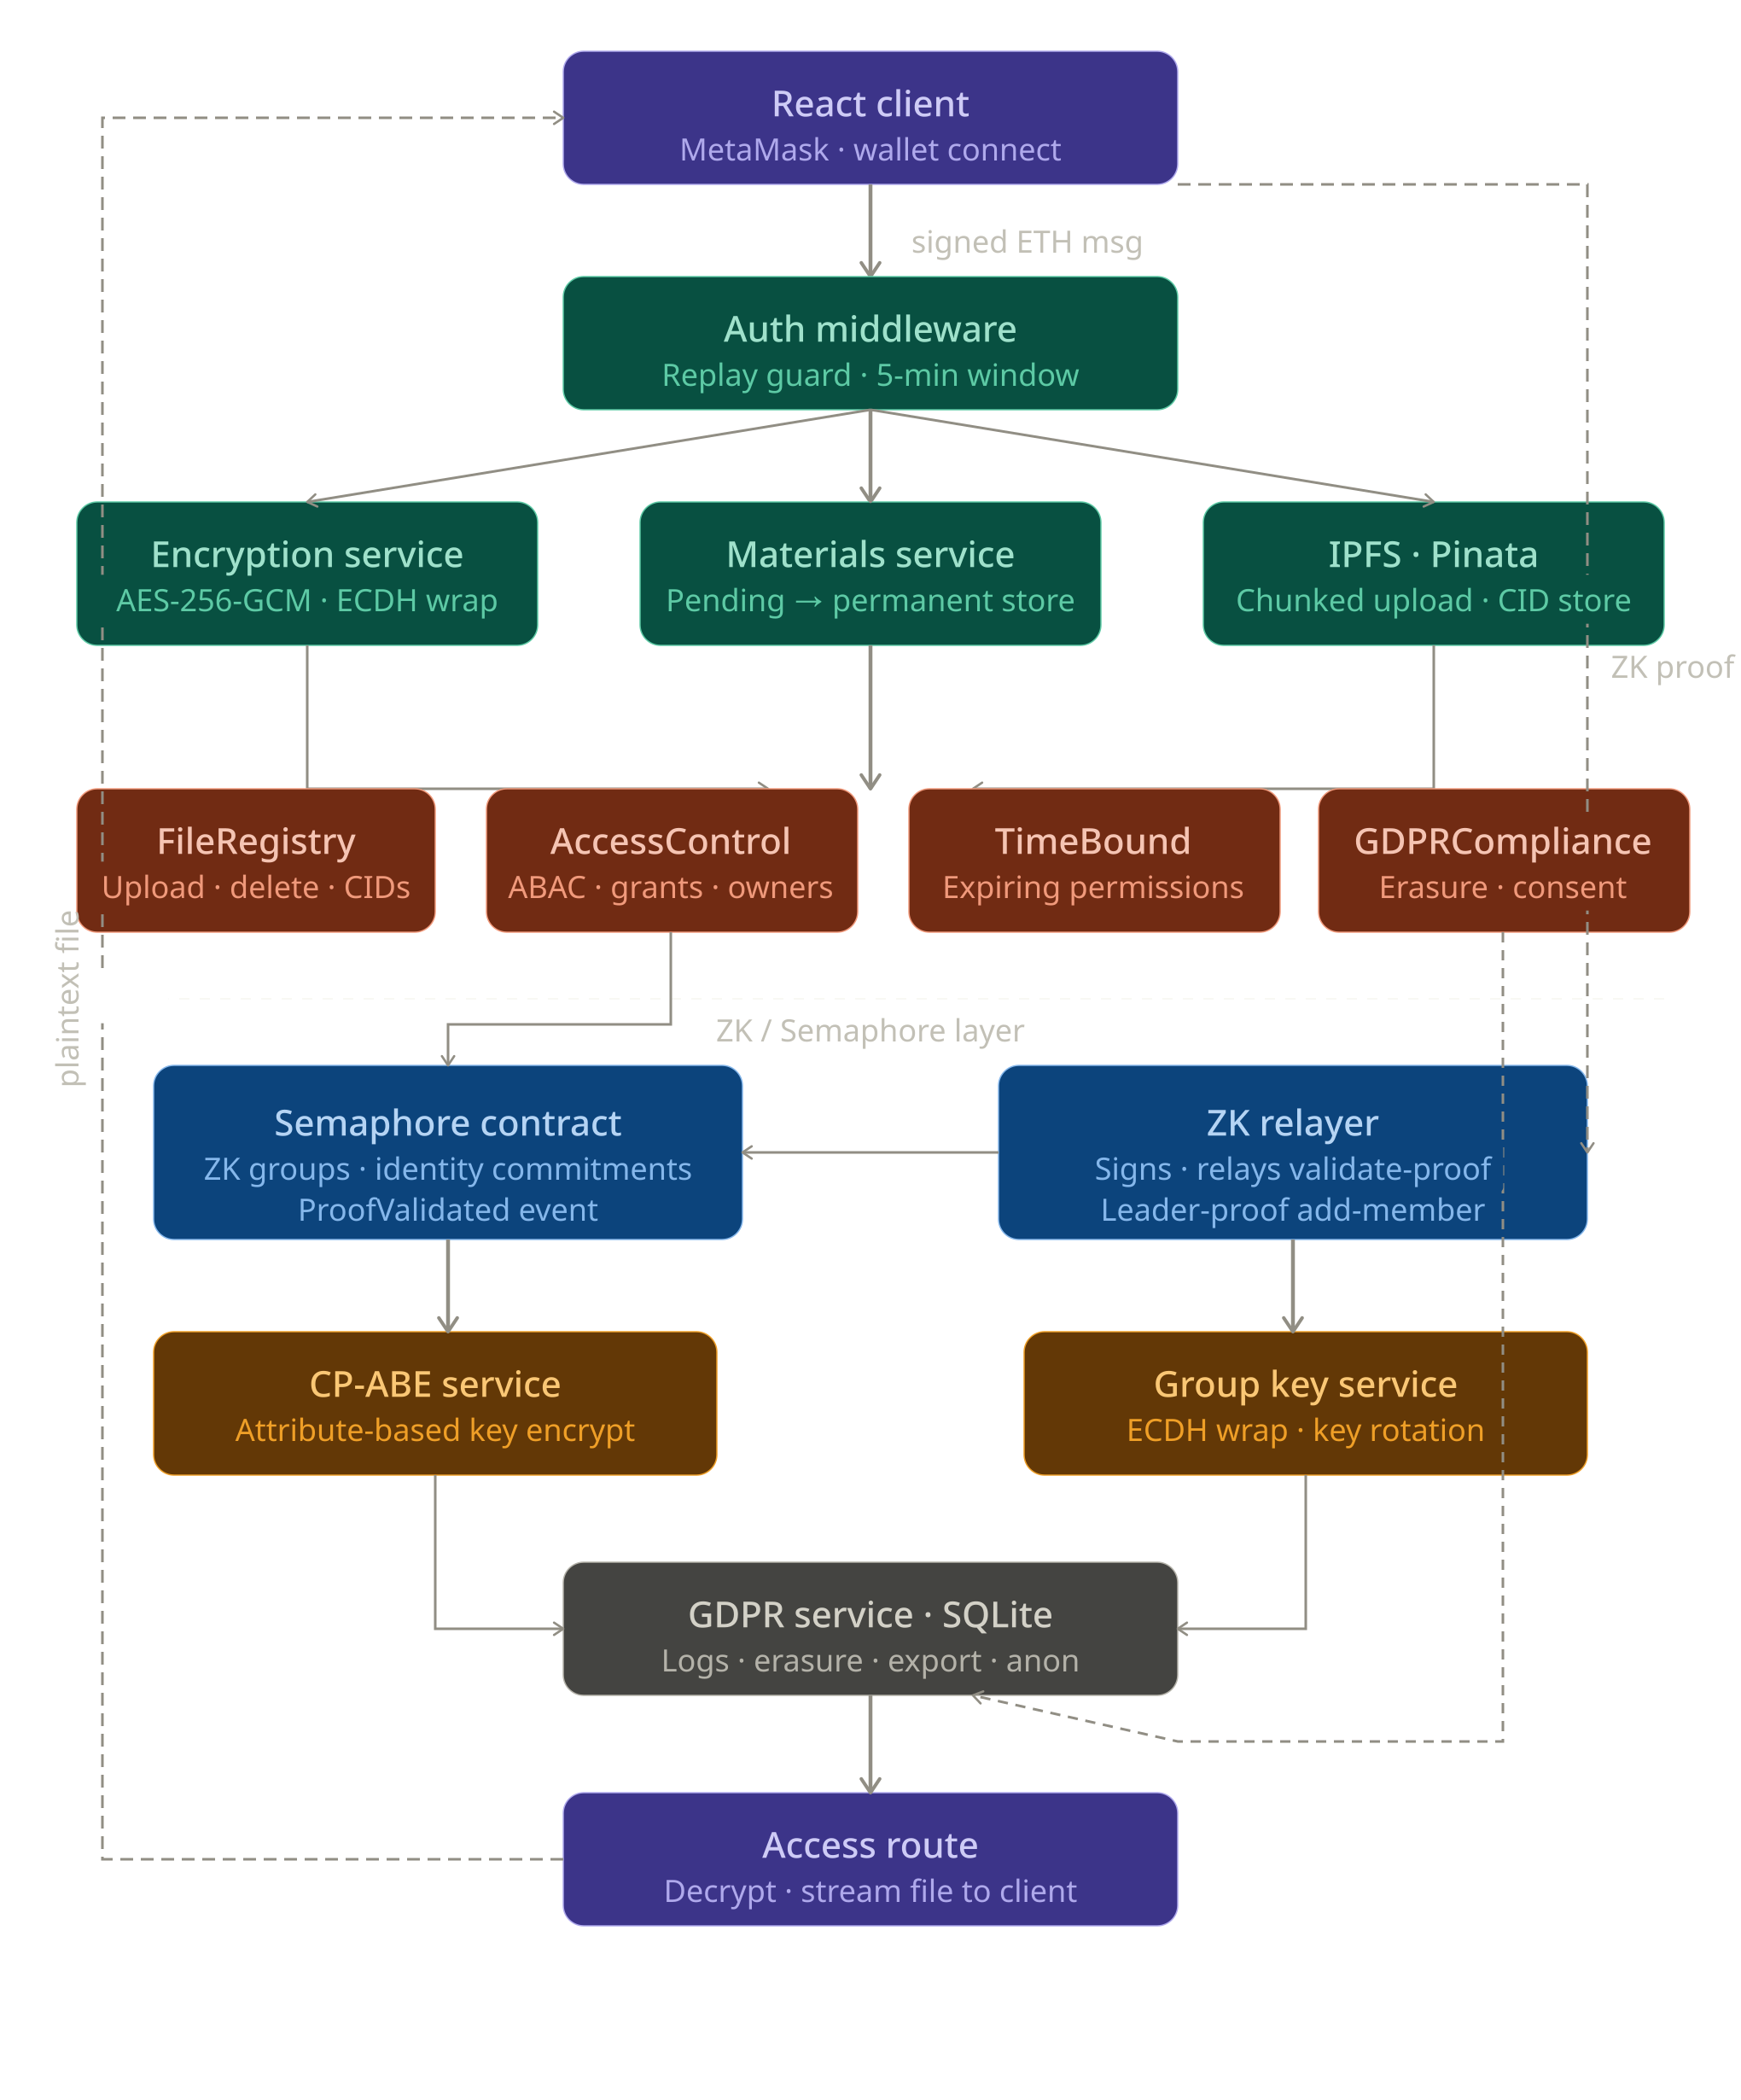
\includegraphics[width=\paperwidth,height=0.96\paperheight,keepaspectratio]{securefile_architecture_flow.png}%
}{%
  \includesvg[width=\paperwidth,height=0.96\paperheight,keepaspectratio]{securefile_architecture_flow}%
}
\end{frame}

% ── Upload & Sharing Workflow ──────────────────────────────────────────────────
\begin{frame}{Upload \& Sharing Workflow}
\centering
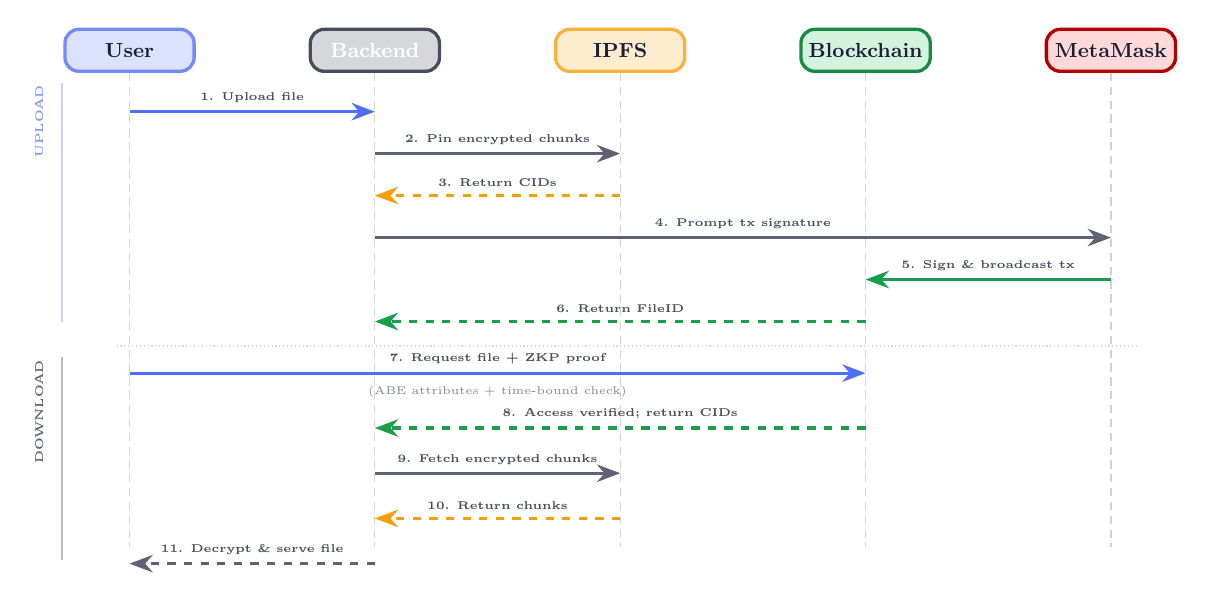
\begin{tikzpicture}[
  actorblue/.style={rectangle, rounded corners=5pt, draw=electricblue!80, very thick,
    fill=electricblue!20, text=navyblue, font=\small\bfseries,
    minimum height=0.65cm, minimum width=2.0cm, align=center},
  actordark/.style={rectangle, rounded corners=5pt, draw=navyblue!80, very thick,
    fill=navyblue!18, text=white, font=\small\bfseries,
    minimum height=0.65cm, minimum width=2.0cm, align=center},
  actororange/.style={rectangle, rounded corners=5pt, draw=warnorange!80, very thick,
    fill=warnorange!20, text=navyblue, font=\small\bfseries,
    minimum height=0.65cm, minimum width=2.0cm, align=center},
  actorgreen/.style={rectangle, rounded corners=5pt, draw=successgreen!70!black, very thick,
    fill=successgreen!20, text=navyblue, font=\small\bfseries,
    minimum height=0.65cm, minimum width=2.0cm, align=center},
  actorred/.style={rectangle, rounded corners=5pt, draw=red!70!black, very thick,
    fill=red!15, text=navyblue, font=\small\bfseries,
    minimum height=0.65cm, minimum width=2.0cm, align=center},
  lbl/.style={font=\tiny\bfseries, text=navyblue!80},
  scale=0.82, transform shape
]

\node[actorblue]   (U)   at (0,0)    {User};
\node[actordark]   (BE)  at (3.8,0)  {Backend};
\node[actororange] (IP)  at (7.6,0)  {IPFS};
\node[actorgreen]  (BC)  at (11.4,0) {Blockchain};
\node[actorred]    (MM)  at (15.2,0) {MetaMask};

\draw[gray!35, densely dashed, thin] (0,-0.35)    -- (0,-7.7);
\draw[gray!35, densely dashed, thin] (3.8,-0.35)  -- (3.8,-7.7);
\draw[gray!35, densely dashed, thin] (7.6,-0.35)  -- (7.6,-7.7);
\draw[gray!35, densely dashed, thin] (11.4,-0.35) -- (11.4,-7.7);
\draw[gray!35, densely dashed, thin] (15.2,-0.35) -- (15.2,-7.7);

\node[font=\tiny\bfseries, text=electricblue!70] at (-1.4,-1.1) {\rotatebox{90}{UPLOAD}};
\draw[electricblue!30, thick] (-1.05,-0.5) -- (-1.05,-4.2);

\draw[-Stealth, very thick, color=electricblue]
  (0,-0.95) -- node[above, lbl] {\textbf{1.} Upload file} (3.8,-0.95);

\draw[-Stealth, very thick, color=navyblue!70]
  (3.8,-1.60) -- node[above, lbl] {\textbf{2.} Pin encrypted chunks} (7.6,-1.60);

\draw[-Stealth, very thick, dashed, color=warnorange]
  (7.6,-2.25) -- node[above, lbl] {\textbf{3.} Return CIDs} (3.8,-2.25);

\draw[-Stealth, very thick, color=navyblue!70]
  (3.8,-2.90) -- node[above, lbl] {\textbf{4.} Prompt tx signature} (15.2,-2.90);

\draw[-Stealth, very thick, color=successgreen!80!black]
  (15.2,-3.55) -- node[above, lbl] {\textbf{5.} Sign \& broadcast tx} (11.4,-3.55);

\draw[-Stealth, very thick, dashed, color=successgreen!80!black]
  (11.4,-4.20) -- node[above, lbl] {\textbf{6.} Return FileID} (3.8,-4.20);

\node[font=\tiny\bfseries, text=navyblue!70] at (-1.4,-5.6) {\rotatebox{90}{DOWNLOAD}};
\draw[navyblue!30, thick] (-1.05,-4.75) -- (-1.05,-7.9);

\draw[gray!30, densely dotted] (-0.2,-4.58) -- (15.6,-4.58);

\draw[-Stealth, very thick, color=electricblue]
  (0,-5.0) -- node[above, lbl] {\textbf{7.} Request file + ZKP proof} (11.4,-5.0);
\node[font=\tiny, text=navyblue!55] at (5.7,-5.28)
  {(ABE attributes + time-bound check)};

\draw[-Stealth, very thick, dashed, color=successgreen!80!black]
  (11.4,-5.85) -- node[above, lbl] {\textbf{8.} Access verified; return CIDs} (3.8,-5.85);

\draw[-Stealth, very thick, color=navyblue!70]
  (3.8,-6.55) -- node[above, lbl] {\textbf{9.} Fetch encrypted chunks} (7.6,-6.55);

\draw[-Stealth, very thick, dashed, color=warnorange]
  (7.6,-7.25) -- node[above, lbl] {\textbf{10.} Return chunks} (3.8,-7.25);

\draw[-Stealth, very thick, dashed, color=navyblue!70]
  (3.8,-7.95) -- node[above, lbl] {\textbf{11.} Decrypt \& serve file} (0,-7.95);

\end{tikzpicture}
\end{frame}

\begin{frame}{New End-Evaluation Features Added Since Mid Review}
\begin{columns}[t]
\column{0.48\textwidth}
\begin{tcolorbox}[bluebox, title=\textbf{ZK/Relayer Enhancements}]
\scriptsize
\begin{itemize}
  \item Relayer endpoints for proof validation, group creation, and member add
  \item Leader-authorized membership add path using nonce + deadline + nullifier checks
  \item Frontend migrated from wallet-direct member add to relayer-backed flow
  \item Backend endpoint to fetch ZK group leader configuration
\end{itemize}
\end{tcolorbox}
\column{0.48\textwidth}
\begin{tcolorbox}[greenbox, title=\textbf{Deployment/Operations Enhancements}]
\scriptsize
\begin{itemize}
  \item Improved deploy script for relayer setup and network handling
  \item Optional Tenderly plugin behavior with virtual-network deployment support
  \item Address synchronization to backend/client artifacts
  \item Better startup validation and safer error handling
\end{itemize}
\end{tcolorbox}
\end{columns}
\end{frame}

\begin{frame}{Post-Mid Deep Dive: ZK Groups, Semaphore, Relayer}
\tiny
\begin{columns}[t]
\column{0.48\textwidth}
\begin{tcolorbox}[bluebox, title=\textbf{What Changed in Group Model}]
\begin{itemize}
  \setlength{\itemsep}{1.5pt}
  \setlength{\parskip}{0pt}
  \setlength{\parsep}{0pt}
  \item ZK groups use \texttt{createZkGroupWithLeader()}.
  \item Leader-auth group is initialized with leader commitment.
  \item Direct \texttt{addZkGroupMember()} is disabled by design.
  \item Member add now requires leader proof + relayer tx.
\end{itemize}
\end{tcolorbox}
\vspace{0.05cm}
\begin{tcolorbox}[greenbox, title=\textbf{Semaphore Verification Semantics}]
\begin{itemize}
  \setlength{\itemsep}{1.5pt}
  \setlength{\parskip}{0pt}
  \setlength{\parsep}{0pt}
  \item Access proof message is bound to \texttt{fileId}.
  \item Leader-add proof binds \texttt{groupId, commitment, nonce, deadline}.
  \item Unique nullifiers block proof replay.
\end{itemize}
\end{tcolorbox}

\column{0.48\textwidth}
\begin{tcolorbox}[orangebox, title=\textbf{Relayer API + Frontend Integration}]
\begin{itemize}
  \setlength{\itemsep}{1.5pt}
  \setlength{\parskip}{0pt}
  \setlength{\parsep}{0pt}
  \item Relayer routes: validate proof, create group, get leader config, add member.
  \item Frontend uses relay helpers for ZK group create/member add.
  \item Leader pre-check config is fetched from backend endpoint.
  \item ZK-public download verifies proof receipt/logs before serving.
\end{itemize}
\end{tcolorbox}
\vspace{0.05cm}
\begin{tcolorbox}[navybox, title=\textbf{Security Outcome}]
Wallet identity is decoupled from proof logic while keeping contract-side checks auditable and strictly validated.
\end{tcolorbox}
\end{columns}
\end{frame}

% =============================================================================
\section{Results \& Analysis}
% =============================================================================

\begin{frame}{Results Summary \& Security Analysis}
\tiny
\begin{columns}[t]
\column{0.48\textwidth}
\begin{tcolorbox}[bluebox, title=\textbf{Smart Contracts Delivered}]
\begin{itemize}
  \setlength{\itemsep}{1.5pt}
  \setlength{\parskip}{0pt}
  \setlength{\parsep}{0pt}
  \item \texttt{FileRegistry.sol} --- CID metadata + soft delete
  \item \texttt{FileAccessControl.sol} --- ABAC, grants/revokes, ZK policy hooks
  \item \texttt{TimeBoundPermissions.sol} --- expiry, extend, revoke
  \item \texttt{GDPRCompliance.sol} --- erasure/compliance signaling
  \item \texttt{Semaphore} integration for anonymous proof verification
\end{itemize}
\end{tcolorbox}
\vspace{0.08cm}
\begin{tcolorbox}[greenbox, title=\textbf{Implemented Security Controls}]
\tiny\centering
Rate limiting $\cdot$ Helmet/CORS hardening $\cdot$ signature auth
$\cdot$ contract address validation $\cdot$ ReentrancyGuard
\end{tcolorbox}
\column{0.48\textwidth}
\begin{tcolorbox}[redbox, title=\textbf{Security Guarantees (Code-backed)}]
\begin{itemize}
  \setlength{\itemsep}{1.5pt}
  \setlength{\parskip}{0pt}
  \setlength{\parsep}{0pt}
  \item \textbf{Confidentiality} --- AES-256-GCM; no plaintext on IPFS
  \item \textbf{Integrity} --- SHA-256 chunk/file hash checks
  \item \textbf{Authentication} --- signed-message API auth + wallet signer
  \item \textbf{Authorization} --- ABAC + grants + timed + ZK policy checks
  \item \textbf{Auditability} --- on-chain events + SQLite ops trail
  \item \textbf{Privacy} --- Semaphore proofs reduce identity disclosure
\end{itemize}
\end{tcolorbox}
\end{columns}
\end{frame}


% ── Thank You Slide ───────────────────────────────────────────────────────────
\begin{frame}[plain]
\begin{tikzpicture}[remember picture, overlay]
  \fill[navyblue] (current page.north west) rectangle (current page.south east);
  \fill[electricblue, opacity=0.18]
    (current page.north east)
    .. controls +(-3,-2) and +(2,2) ..
    ([xshift=-3cm]current page.east)
    -- (current page.south east) -- cycle;
\end{tikzpicture}
\vspace{2.2cm}
\centering
{\Huge\textbf{\textcolor{white}{Thank You}}}\\[0.5cm]


\end{frame}

% =============================================================================
\end{document}
